% Figure Q2 hero prototype : generated by experiments/q2_convergence_trajectories.py --hero.
% Preview-only; not yet linked from the main manuscript.
\begin{figure}[t]
 \centering
 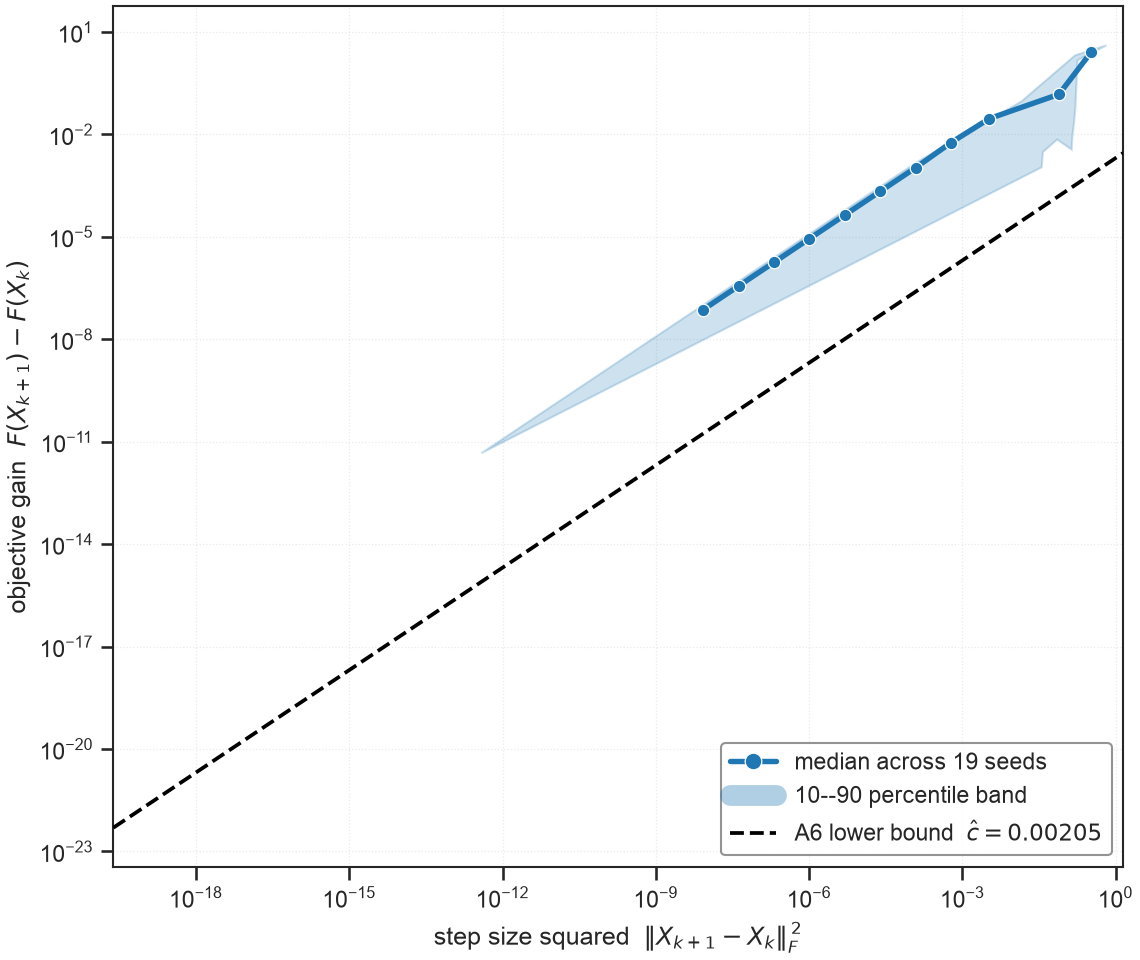
\includegraphics[width=0.78\linewidth]{../shared/figures/generated/q2_convergence_trajectories_hero.png}
 \caption{\textbf{Q2 hero: empirical witness of Lemma~\ref{lem:a-sufficient-ascent} (A6).} Scatter of per-iterate pairs $(\|X_{k+1}-X_k\|_F^{\,2},\ F(X_{k+1}) - F(X_k))$ across every iteration of every replicate in Figure~\ref{fig:q2-trajectories}; marker colour identifies the replicate seed (legend). The dashed black line is $y = \hat c \cdot x$ with $\hat c$ the smallest empirically observed ratio across the full trajectory, so every point lies on or above it by construction. The slope-1 envelope is Lemma~\ref{lem:a-sufficient-ascent} made visual: the sufficient-ascent inequality is \emph{tight} on this experiment, with $c_1 \geq \hat c$ in \eqref{eq:a-sufficient-ascent}.}
 \label{fig:q2-trajectories-hero}
\end{figure}
